% Created with jtex v.1.0.1
\documentclass{article}
\usepackage{arxiv}

\usepackage[utf8]{inputenc} % allow utf-8 input
\usepackage[T1]{fontenc}    % use 8-bit T1 fonts
\usepackage{hyperref}       % hyperlinks
\usepackage{url}            % simple URL typesetting
\usepackage{datetime}       % show dates in the title block
\usepackage{booktabs}       % professional-quality tables
\usepackage{amsfonts}       % blackboard math symbols
\usepackage{nicefrac}       % compact symbols for 1/2, etc.
\usepackage{microtype}      % microtypography
\usepackage{graphicx}
\usepackage{natbib}
\usepackage{doi}
\usepackage{xcolor}

%%%%%%%%%%%%%%%%%%%%%%%%%%%%%%%%%%%%%%%%%%%%%%%%%%
%%%%%%%%%%%%%%%%%%%%  imports  %%%%%%%%%%%%%%%%%%%
\usepackage{amsmath}
%%%%%%%%%%%%%%%%%  math commands  %%%%%%%%%%%%%%%%
\newcommand{\DiscFac}{\beta}
\newcommand{\cFunc}{\mathrm{c}}
\newcommand{\uFunc}{\mathrm{u}}
\newcommand{\vFunc}{\mathrm{v}}
\newcommand{\Alive}{\mathcal{L}}
\newcommand{\h}{h}
\newcommand{\cLvl}{\mathbf{c}}
\newcommand{\mLvl}{\mathbf{m}}
\newcommand{\pLvl}{\mathbf{p}}
\newcommand{\Ex}{\mathbb{E}}
\newcommand{\CRRA}{\rho}
\newcommand{\PermGroFac}{\pmb{\Phi}}
\newcommand{\Rfree}{\mathsf{R}}
\newcommand{\PermShk}{\mathbf{\Psi}}
\newcommand{\TranShk}{\pmb{\xi}}
\newcommand{\aNrm}{a}
\newcommand{\cNrm}{c}
\newcommand{\RNrm}{\mathcal{R}}
\newcommand{\TranShkEmp}{\pmb{\theta}}
\newcommand{\mNrm}{m}
\newcommand{\pZero}{\wp}
\newcommand{\aFunc}{\mathrm{a}}
\newcommand{\kapShare}{\alpha}
\newcommand{\wealth}{o}
\newcommand{\kap}{k}
\newcommand{\wealthShare}{\delta}
\newcommand{\wFunc}{\mathrm{w}}
\newcommand{\aRat}{a}
\newcommand{\mRat}{m}
\newcommand{\aMat}{[\mathrm{a}]}
\newcommand{\mMat}{[\mathrm{m}]}
\newcommand{\weight}{\omega}
%%%%%%%%%%%%%%%%%%%%%%%%%%%%%%%%%%%%%%%%%%%%%%%%%%

\hypersetup{colorlinks = true,
linkcolor = purple,
urlcolor  = blue,
citecolor = cyan,
anchorcolor = black}

\title{Structural Estimation of Life Cycle Models with Wealth in the Utility Function}

\newdate{articleDate}{16}{7}{2023}
\date{\displaydate{articleDate}}

\makeatletter
\let\@fnsymbol\@arabic
\makeatother

\author{Alan Lujan\footnotemark[1]\\
Ohio State University\\Econ-ARK\\}

% Uncomment to override  the `A preprint' in the header
\renewcommand{\headeright}{Economics}
\renewcommand{\undertitle}{}
\renewcommand{\shorttitle}{Structural Estimation}

%% Add PDF metadata to help others organize their library
%% Once the PDF is generated, you can check the metadata with
%% $ pdfinfo template.pdf
\hypersetup{
pdftitle={\@title},
pdfsubject={},
pdfauthor={\@author},
pdfkeywords={structural estimation,life cycle,wealth in the utility},
addtopdfcreator={Written in Curvenote}
}

\begin{document}
\maketitle
\footnotetext[1]{Correspondence to: alanlujan91@gmail.com}

\begin{abstract}
Heterogeneous Agent Models (HAM) are a powerful tool for understanding the effects of monetary and fiscal policy on the economy. However, current state-of-the-art frameworks such as Heterogeneous Agent New Keynesian (HANK) models have limitations that hinder their ability to accurately replicate real-world economic phenomena. Specifically, HANK models struggle to account for the observed accumulation of wealth at the very top of the distribution and lack important life cycle properties such as time-varying preferences, mortality, and income risk. On the one hand, the inability to pin down wealth at the tail of the distribution has been a problem for HANK models precisely because it has implications for the transmission of monetary and fiscal policy. On the other hand, agents in HANK are generally conceived as perpetual youth with infinite horizons and without age-specific profiles of mortality and income risk. This is problematic as it ignores the effects of these policies on potentially more affected communities, such as young families with children or the low-wealth elderly. In this paper, I investigate the effects of both life cycle considerations as well as wealth in the utility on the structural estimation of HAMs. Structural estimation is the first step in evaluating the effect of monetary and fiscal policies in a HANK framework, and my hope is that this paper will lead to better models of the economy that can be used to inform policy.
\end{abstract}

\keywords{structural estimation, life cycle, wealth in the utility}

I would like to thank my advisor, Chris Carroll, for his guidance and support throughout this project. His expertise and mentorship have been invaluable in shaping my work. Additionally, I would like to extend my appreciation to the members of the \href{https://econ-ark.org/}{Econ-ARK} team for fostering a dynamic and collaborative community that has greatly enriched my experience. Their contributions and feedback have been instrumental in helping me achieve my goals. All remaining errors are my own. The figures in this paper were generated using the \href{https://github.com/econ-ark/HARK}{Econ-ARK/HARK} toolkit.

\section{Introduction}\label{Introduction}

Increased computational power has allowed economists to focus on more complex models of household consumption and saving. In particular, Heterogeneous Agent Models (HAM) have become a popular tool to analyze households' response to aggregate economic shocks in the face of uncertainty. Nevertheless, current state-of-the-art models have struggled to replicate the distribution of wealth at the very top of the distribution and the extent of wealth inequality. A new class of models, the Heterogeneous Agent New Keynesian (HANK) models, have taken the literature by storm and become the standard for analyzing the effects of monetary and fiscal policy\footnote{See \cite{Kaplan_2018}, \cite{Acharya_2020}, \cite{Ravn_2020}, and \cite{Auclert_2020}, among others.}. Even HANK models, however, inherit the inability to capture the distribution of wealth from their predecessors. Moreover, they also lack important life cycle properties such as time-varying preferences, household composition, and mortality and income risk. These limitations make the workhorse HANK models ill-suited for analyzing the effects of economic shocks and policy on the spectrum of households in the economy, from young families with children to retirees, and in particular, on the most vulnerable households among these subgroups. In this paper, I investigate the effects of both life cycle considerations as well as wealth in the utility on the structural estimation of HAMs. Thorough this effort, we hope to contribute to the development of better models of the economy that can be used to inform policy.

\cite{Carroll_1998} demonstrates that the rich have higher lifetime savings rates\footnote{See also \cite{Dynan_2004}.} which can not be explained by models of consumption smoothing and precautionary savings alone. Instead, he argues that the simplest model that accounts for this is one with wealth in the utility function. This is because households either derive utility from the accumulation wealth itself or wealth provides a flow of services such as political power and social status. In either case, this pattern of higher savings can be modeled by putting wealth directly in the utility function. In his paper, he proposes the use of additively separable utility of wealth and consumption\footnote{Also see \cite{Carroll_2000}, which uses additively separable utility of wealth and consumption to explain the portfolio choices of the rich.}, which we will explore in this paper. Additionally, however, we will also explore the use of non-separable utility of consumption and wealth. With non-separability of utility, we obtain a model that allows for a marginal utility of consumption that is increasing in wealth even while it is decreasing in consumption. This dynamic complementarity between consumption and wealth is a key feature of our model that induces a strong savings motive for the rich.

Wealth Inequality has been a persistent problem for the HAM literature\footnote{See \cite{Cagetti_2008}, \cite{De_Nardi_2015}, \cite{De_Nardi_2017}, for surveys on the topic.}. Models with entrepreneurship, preference heterogeneity, habit formation, bequest motives, human capital, and large earnings risk have had varying degrees of success in replicating the distribution of wealth. However, these models have been unable to account for the fat tail in the distribution. Recent research highlights the importance of savings among the richest in the United States and its distributional effects. \cite{Mian_2020} find that the rise in savings by the richest households in the U.S. over the last 40 years is strongly associated with dissaving by the non-rich and the government, in the form of debt, which might have implications for the rise in household debt and declining interest rates in the last few decades. Similarly, \cite{Auclert_2023} find that as non-rich households spend down their excess savings, the incomes of the rich rise, which in turns leads to an increase in their excess savings. This movement of savings across the distribution leads to a prolonged increase in aggregate demand and can dampen the effects of monetary policy. \cite{Michaillat_2021} present a similar model within the HANK literature that includes wealth in the utility function. However, because this paper uses continuous time methods, it is unable to capture the life cycle properties of more realistic models.

The purpose of this paper is to investigate the effects of wealth in the utility function as well as life-cycle properties on the structural estimation of HAMs. By using wealth in the utility function, we can better match the top of the wealth distribution and the motives for wealth accumulation. Also, by parameterizing a rich model of life cycle properties such as age-specific and household-size-adjusted preferences, and mortality and income risk, we can better understand the effects that economic shocks and policies have on young working families, workers saving toward retirement, and retirees. In particular, we can better understand the effects of monetary policy on the distribution of wealth and consumption across the life cycle.

The remainder of the paper is organized as follows. Section 2 provides the baseline models and alternative specifications with wealth in the utility function. Section 3 describes the solution methods used to solve these models. Section 4 describes the quantitative strategy used to calibrate and estimate the models, followed by sensitivity analysis of the results. Finally, Section 5 contains closing remarks and future directions.

\section{Life Cycle Incomplete Markets Models}\label{Life Cycle Incomplete Markets Models}

An important extension to the Standard Incomplete Markets (SIM) model is the Life Cycle Incomplete Markets (LCIM) model as in \cite{Cagetti_2003}, \cite{Gourinchas_2002}, and \cite{Palumbo_1999}, among others. The LCIM model is a natural extension to the SIM model that allows for age-specific profiles of preferences, mortality, and income risk.

\subsection{The Baseline Model}\label{The Baseline Model}

The agent's objective is to maximize present discounted utility from consumption over the life cycle with a terminal period of $T$:

\begin{equation}
\label{eq:lifecyclemax}
\vFunc_{t}(\pLvl_{t},\mLvl_{t})  =    \max_{\{\cFunc\}_{t}^{T}} ~ \uFunc(\cLvl_{t})+\Ex_{t}\left[\sum_{n=1}^{T-t} {\beth}^{n} \Alive_{t}^{t+n}\hat{\DiscFac}_{t}^{t+n} \uFunc(\cLvl_{t+n}) \right]
\end{equation}

where $\pLvl_{t}$ is the permanent income level, $\mLvl_{t}$ is total market resources, $\cLvl_{t}$ is consumption, and

\begin{equation}
\begin{align}
    \beth & :  \text{time-invariant `pure' discount factor}
    \\ \Alive _{t}^{t+n} & :  \text{probability to }\Alive\text{ive until age $t+n$ given alive at age $t$}
    \\ \hat{\DiscFac}_{t}^{t+n} & :  \text{age-varying discount factor between ages $t$ and $t+n$.}
\end{align}
\end{equation}

It will be convenient to work with the problem in permanent-income-normalized form as in \cite{Carroll_2004}, which allows us to reduce a 2 dimensional problem of permanent income and wealth into a 1 dimensional problem of wealth normalized by permanent income. The recursive Bellman equation can be expressed as:

\begin{equation}
\begin{align}
    {\vFunc}_{t}({m}_{t}) & = \max_{\cNrm_{t}} ~ \uFunc(\cNrm_{t})+\beth\Alive_{t+1}\hat{\DiscFac}_{t+1}
    \Ex_{t}[(\PermShk_{t+1}\PermGroFac_{t+1})^{1-\CRRA}{\vFunc}_{t+1}({m}_{t+1})]
    \\ & \text{s.t.} & 
    \\ \aNrm_{t} & = {m}_{t}-\cNrm_{t} 
    \\ {m}_{t+1} & = \aNrm_{t}\underbrace{\left(\frac{\Rfree}{\PermShk_{t+1}\PermGroFac_{t+1}}\right)}_{\equiv \RNrm_{t+1}}
    + ~\TranShkEmp_{t+1}
\end{align}
\end{equation}

where $\cNrm$, $\aNrm$, and $\mNrm$ are consumption, assets, and market resources normalized by permanent income, respectively, $\vFunc$ and $\uFunc$ are now the normalized value and utility functions,  and

\begin{equation}
\begin{align}
  \PermShk_{t+1} & :  \text{mean-one shock to permanent income}
    \\ \PermGroFac_{t+1} & :  \text{permanent income growth factor}
    \\ \TranShkEmp_{t+1} & :  \text{transitory shock to permanent income}
    \\ \RNrm_{t+1} & :  \text{permanent income growth normalized return factor}
\end{align}
\end{equation}

with all other variables are defined as above. The transitory and permanent shocks to income are defined as:

\begin{equation}
\begin{align}
\TranShkEmp_{s}  = &
    \begin{cases}
        0\phantom{/\pZero} & \text{with probability $\pZero>0$}
        \\ \xi_{s}/\pZero & \text{with probability $(1-\pZero)$, where
            $\log \xi_{s}\thicksim \mathcal{N}(-\sigma_{[\xi, t]}^{2}/2,\sigma_{[\xi, t]}^{2})$}
    \end{cases}
    \\ \phantom{/\pZero} \\ & \text{and }  \log \PermShk_{s}   \thicksim \mathcal{N}(-\sigma_{[\PermShk, t]}^{2}/2,\sigma_{[\PermShk, t]}^{2}).
  \end{align}
\end{equation}

\subsection{Wealth in the Utility Function}\label{Wealth in the Utility Function}

A simple extension to the Life Cycle Incomplete Markets (LCIM) model is to include wealth in the utility function. \cite{Carroll_1998} argues that models in which the only driver of wealth accumulation is consumption smoothing are not consistent with the saving behavior of the wealthiest households. Instead, they propose a model in which households derive utility from their level of wealth itself or they derive a flow of services from political power and social status, calling it the `Capitalist Spirit' model. In turn, we can add this feature to the LCIM model by adding a utility function with consumption and wealth. We call this the Wealth in the Utility Function Incomplete Markets (WUFIM) model.

\begin{equation}
\begin{align}
    {\vFunc}_{t}({m}_{t}) & = \max_{\cNrm_{t}} ~ \uFunc(\cNrm_{t}, \aNrm_{t})+\beth\Alive_{t+1}\hat{\DiscFac}_{t+1}
    \Ex_{t}[(\PermShk_{t+1}\PermGroFac_{t+1})^{1-\CRRA}{\vFunc}_{t+1}({m}_{t+1})]
    \\ & \text{s.t.} & 
    \\ \aNrm_{t} & = {m}_{t}-\cNrm_{t} 
    \\ {m}_{t+1} & = \aNrm_{t}\RNrm_{t+1}+ ~\TranShkEmp_{t+1}
\end{align}
\end{equation}

\textbf{Separable Utility} \cite{Carroll_1998} presents extensive empirical and informal evidence for a LCIM model with wealth in the utility function. Specifically, the paper uses a utility that is separable in consumption and wealth:

\begin{equation}
\uFunc(\cNrm_{t}, \aNrm_{t}) = \frac{\cNrm_{t}^{1-\CRRA}}{1-\CRRA}
    + \kapShare_{t} \frac{(\aFunc_{t} - \underline\aNrm)^{1-\wealthShare}}{1-\wealthShare}
\end{equation}

where $\kapShare$ is the relative weight of the utility of wealth and $\wealthShare$ is the relative risk aversion of wealth.

\textbf{Non-separable Utility} A different model that we will explore is one in which the utility function is non-separable in consumption and wealth; i.e. consumption and wealth are complimentary goods. In the case of the LCIM model, this dynamic complementarity drives the accumulation of wealth not only for the sake of wealth itself, but also because it increases the marginal utility of consumption.

\begin{equation}
\uFunc(\cNrm_{t}, \aNrm_{t}) = \frac{(\cNrm_{t}^{1-\wealthShare} (\aNrm_{t} - \underline\aNrm)^\wealthShare)^{1-\CRRA}}{(1-\CRRA)}
\end{equation}

\section{Solution Methods}\label{Solution Methods}

For a brief departure, let's consider how we solve these problems generally. Define the post-decision value function as:

\begin{equation}
\begin{align}
    \DiscFac_{t+1} \wFunc_{t}(\aNrm_{t}) & = \beth\Alive_{t+1}\hat{\DiscFac}_{t+1}
    \Ex_{t}[(\PermShk_{t+1}\PermGroFac_{t+1})^{1-\CRRA}{\vFunc}_{t+1}({m}_{t+1})]
    \\ & \text{s.t.}
    \\ {m}_{t+1} & = \aNrm_{t}\RNrm_{t+1}+ ~\TranShkEmp_{t+1}
\end{align}
\end{equation}

For our purposes, it will be useful to simplify the notation a bit by dropping time subscripts. The recursive problem can then be written as:

\begin{equation}
\begin{align}
    \vFunc(\mRat) & = \max_{\cNrm} ~ \uFunc(\cNrm, \aNrm) + \DiscFac \wFunc(\aRat)
    \\ & \text{s.t.}
    \\ \aNrm & = \mRat-\cNrm
\end{align}
\end{equation}

\subsection{Endogenous Grid Method, Abridged}\label{Endogenous Grid Method, Abridged}

In the standard incomplete markets (SIM) model, the utility function is simply $\uFunc(\cNrm)$ and the Euler equation is $\uFunc'(\cNrm) = \DiscFac \wFunc'(\aNrm)$, which is a necessary and sufficient condition for an internal solution of the optimal choice of consumption. If $\uFunc(\cNrm)$ is differentiable and its marginal utility is invertible, then the Euler equation can be inverted to obtain the optimal consumption function as $\cNrm(\aNrm) = \uFunc'^{ -1}(\DiscFac \wFunc'(\aNrm))$. Using an \textit{exogenous} grid of post-decision savings $\aMat$, we can obtain an \textit{endogenous} grid of market resources $\mMat$ by using the budget constraint $\mNrm(\aMat) = \aMat + \cNrm(\aMat)$ such that this collection of grids satisfy the Euler equation. This is the endogenous grid method (EGM) of \cite{Carroll_2006}.

In the presence of wealth in the utility function, the Euler equation is more complicated and may not be invertible in terms of optimal consumption. Consider the first order condition for an optimal combination of consumption and savings, denoted by $^*$:

\begin{equation}
\uFunc_{c}'(\cNrm^*, \aNrm^*) - \uFunc_{a}'(\cNrm^*, \aNrm^*) = \DiscFac \wFunc'(\aNrm^*)
\end{equation}

If the utility of consumption and wealth is additively separable, then the Euler equation can be written as $\uFunc_{c}'(\cNrm) = \uFunc_{a}'(\aNrm) + \DiscFac \wFunc'(\aNrm)$. This makes sense, as the agent will equalize the marginal utility of consumption with the marginal utility of wealth today plus the discounted marginal value of wealth tomorrow. In this case, the EGM is simple: we can invert the Euler equation to obtain the optimal consumption policy as $\cNrm(\aNrm) = \uFunc_{c}'^{ -1}\big(\uFunc_{a}'(\aNrm) + \DiscFac \wFunc'(\aNrm)\big)$. We can proceed with EGM as usual, using the budget constraint to obtain the endogenous grid of market resources $\mNrm(\aMat) = \aMat + \cNrm(\aMat)$.

\subsection{Root Finding}\label{Root Finding}

When the utility of consumption and wealth is not additively separable, the Euler equation is not analytically invertible for the optimal consumption policy. The usual recourse is to use a root-finding algorithm to obtain the optimal consumption policy for each point on the grid of market resources, which turns out to be more efficient than grid search maximization.

Holding $\mNrm$ constant, we can define a function $f_{m}$ as the difference between the marginal utility of consumption and the marginal utility of wealth:

\begin{equation}
f_{m}(\cNrm) = \uFunc_{c}'(\cNrm, \mNrm - \cNrm) - \uFunc_{a}'(\cNrm, \mNrm - \cNrm) - \DiscFac \wFunc'(\mNrm - \cNrm)
\end{equation}

The optimal consumption policy is the value of $\cNrm$ that satisfies $f_{m}(\cNrm) = 0$. We can use a root-finding algorithm to obtain the optimal consumption policy for each point on the grid of market resources. Although this is more efficient than grid search maximization, it is still computationally expensive. Unlike the single-step EGM, root finding requires a number of iterations to find the optimal consumption policy, which makes it relatively slower. Nevertheless, we can use clever tricks to speed up the process. One such trick used in this paper is to use the optimal consumption policy from the previous iteration as the initial guess for the next iteration. This is possible because the optimal consumption policy is a continuous function of the grid of market resources and the optional decision from one period to the next is not too different. This is the method used in the code for this paper.

\section{Quantitative Strategy}\label{Quantitative Strategy}

This section describes the quantitative strategy used for calibrating and estimating the Life Cycle Incomplete Markets model with and without Wealth in the Utility Function, following the works of \cite{Cagetti_2003}, \cite{Palumbo_1999}, \cite{Gourinchas_2002}, and \cite{Sabelhaus_2010}, among others. The main objective is to find a set of parameters that can best match the empirical moments of some real-life data using simulation.

\subsection{Calibration}\label{Calibration}

The calibration of the Life Cycle Incomplete Markets model necessitates a richness not present in the SIM model precisely because we are interested in the heterogeneity of agents across different stages of the life cycle, such as the early working period, parenthood, saving for retirement, and retirement. To calibrate this model, we need to identify important patterns in preferences, mortality, and income risk across the life cycle. The first and perhaps most important departure from SIM is that life is finite and agents don't life forever; moreover, the terminal age is not certain as the probability of staying alive decreases with age. In this model, households start their life cycle at age $t = 25$ and live with certainty until retirement at age $t = 65$. After retirement, the probability of staying alive decreases with age, and the terminal age is set to $t = 91$. During their early adulthood, their utility of consumption might need to be adjusted by the arrival and subsequent departure of children. This is handled by a `household-size-adjusted' discount factor that is greater than 1.0 in the presence of children. This is the rationale for parameters $\Alive_{t}$ and $\hat{\DiscFac}_{t}$ in the model, whose values we take from \cite{Cagetti_2003} directly.

The unemployment probability is taken from \cite{Carroll_1992} to be $\pZero = 0.5$ which represents a long run equilibrium of 5\% unemployment in the United States. The remaining life cycle attributes for the distribution of shocks to income ($\PermGroFac_{t}, \ \sigma_{[\PermShk, t]}, \ \sigma_{[\xi, t]}$) are taken from \cite{Sabelhaus_2010}. In their paper, they analyze the variability of labor earnings growth rates between the 80's and 90's and find evidence for the ``Great Moderation'', a decline in variability of earnings across all age groups.

After careful calibration based on the Life Cycle Incomplete Markets literature, we can structurally estimate the remaining parameters $\beth$ and $\CRRA$ to match specific empirical moments of the wealth distribution.

\subsection{Estimation}\label{Estimation}

Structural estimation consists of finding the set of parameters that, when used to solve and simulate the model, result in simulated moments that are as close as possible to the empirical moments observed in the data. For this exercise, we focus on matching the median of the wealth to permanent income ratio for 7 age groups starting from age 25-30 up to age 56-60. The data is aggregated from the waves of the Survey of Consumer Finances (SCF). Matching the median has been standard in the literature precisely because it has been so difficult to match the mean of the wealth distribution given the high degree of wealth inequality in the United States. The Wealth in the Utility Function models however are constructed to better match the dispersion of wealth accumulation, and in future work we will attempt to match the mean of the wealth distribution as well.

Given an initial vector of parameters $\Theta_0 = \{\beth_0, \CRRA_0 \}$, the first step in the estimation procedure is to solve for the steady state of the model. As this is a life cycle exercise, the strategy is to start from the terminal period and work backwards to the initial period. This is known as backward induction. The terminal period is characterized by simple decisions over consumption and bequest, as the agent is certain to die and has no continuation value and thus no use for savings. Having constructed the terminal policy functions and their corresponding value and marginal value, we can solve for the optimal policies in the second to last period using the methods described in the previous section. We can then continue this process until we arrive at the initial period. In the end, and unlike in the SIM model, we have a complete set of policy functions for consumption and saving for every age of the life cycle.

Having solved the steady state of the model for the given set of parameters, we can now use the optimal policy functions to generate simulated data of consumption and savings over the life cycle. We can then calculate the simulated moments of the wealth distribution at the 7 age groups. We can define the objective function as

\begin{equation}
\label{eq:naivePowell}
g(\Theta) =  \sum_{\tau=1}^{7} \weight_{\tau} |\varsigma^{\tau} -\mathbf{s}^{\tau}(\Theta)|
\end{equation}

where $\varsigma^{\tau}$ is the empirical moment of the wealth distribution at age $\tau$, $\mathbf{s}^{\tau}(\Theta)$ is the simulated moment of the wealth distribution at age $\tau$ for a given set of parameters $\Theta$, and $\weight_{\tau}$ is the population weight for a particular age group in our data. The goal is thus to minimize the objective function by choice of $\Theta$ such that  $\hat{\Theta} = \arg \min_{\Theta} g(\Theta)$. To find $\hat{\Theta}$, we use the Nelder-Mead algorithm which uses a simplex method and does not require derivatives of the objective function. This consists of trying a significant number of guesses for $\Theta$, solving the model, and simulating moments which can be quite computationally intensive. Future work will focus on using more efficient methods such as those presented by \cite{Auclert_2021}, where the Jacobian (partial first derivatives) of the objective function is used to find the optimal parameters $\hat{\Theta}$ more efficiently and quickly.

\begin{table}
\centering
\caption{LCIM Estimation Results}
\label{LCIMestimation}
\begin{tabular}{p{\dimexpr 0.500\linewidth-2\tabcolsep}p{\dimexpr 0.500\linewidth-2\tabcolsep}}
\toprule
$\beth$ & $\CRRA$ \\
\hline
0.878 & 3.516 \\
(0.0018) & (0.0266) \\
\bottomrule
\end{tabular}
\end{table}

\textbf{Results for LCIM model} We can see the estimated parameters for the LCIM model in Table~\ref{LCIMestimation}. The estimated values for $\beth$ and $\CRRA$ are 0.878 and 3.1516, respectively, with standard errors estimated via the bootstrap. Additionally, Figure~\ref{fig:IndShockSMMcontour} shows a contour plot of the objective function for the structural estimation exercise where the red star represents the estimated parameters. The contour plot shows that the objective function has a  relatively flat region around the estimated parameters that extends toward higher values of $\CRRA$ and lower values of $\beth$, showing the trade-offs between the estimation of these two parameters.

\begin{figure}[!htbp]
\centering
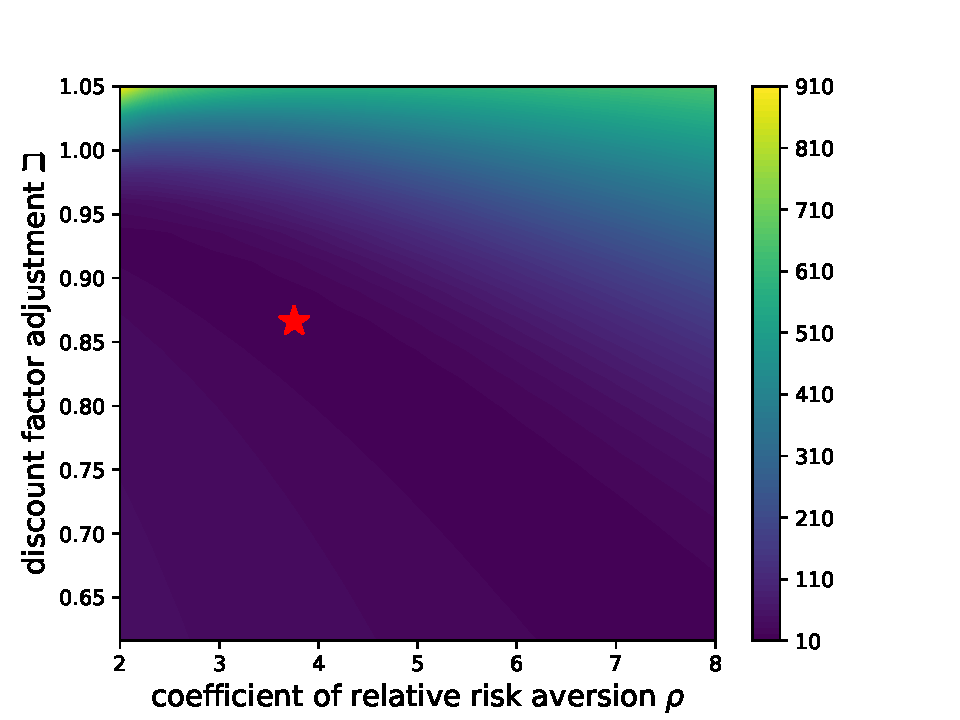
\includegraphics[width=0.7\linewidth]{files/IndShockSMMcontour-f950f8faf8926e47605d36d01964a2f6.pdf}
\caption{Contour plot of the objective function for the structural estimation of the Life Cycle Incomplete Markets model. The red dot represents the estimated parameters.}
\label{fig:IndShockSMMcontour}
\end{figure}

\begin{table}
\centering
\caption{WUFIM Estimation Results}
\label{WUFIMestimation}
\begin{tabular}{p{\dimexpr 0.333\linewidth-2\tabcolsep}p{\dimexpr 0.333\linewidth-2\tabcolsep}p{\dimexpr 0.333\linewidth-2\tabcolsep}}
\toprule
Model & $\beth$ & $\CRRA$ \\
\hline
LCIM w/ Portfolio Choice & 0.866 & 3.756 \\
 & (0.0011) & (0.0313) \\
Separable WUFIM & 0.876 & 3.506 \\
 & (0.0012) & (0.0254) \\
Separable WUFIM w/ Portfolio & 0.864 & 3.806 \\
 & (0.0012) & (0.0263) \\
Non-Separable WUFIM & 0.601 & 5.032 \\
 & (0.0026) & (0.0634) \\
\bottomrule
\end{tabular}
\end{table}

\textbf{Results for WUFIM models} We can see the estimated parameters for our alternative specifications of the LCIM with Wealth in the Utility Function (WUFIM) in Table~\ref{WUFIMestimation}. The estimated values for $\beth$ and $\CRRA$ are 0.866 and 3.756, respectively, for the LCIM with portfolio choice, 0.876 and 3.506, respectively, for the separable WUFIM, 0.864 and 3.806, respectively, for the separable WUFIM with portfolio choice, and 0.601 and 5.032, respectively, for the non-separable WUFIM. The standard errors are estimated via the bootstrap. Additionally, Figure~\ref{fig:AllSMMcontour} shows a contour plot of the objective function for the structural estimation exercise where the red star represents the estimated parameters. From these results, a clear pattern emerges which is worth discussion and further analysis. The estimated parameters for the Separable WUFIM model are not very different from those in LCIM model, which perhaps points at the inability of warm glow bequest models to resolve many of the issues of the SIM and LCIM model. The separable WUFIM model does not produce significant differences in the accumulation of wealth over the life cycle beyond a simple shifting out of the savings function. When we add a portfolio choice to either model, the pure discount factor $\beth$ becomes slightly lower and the coefficient of risk aversion $\CRRA$ increases by a few decimal points. This is because, as the portfolio choice model exposes agents to more risk, they become both more risk averse and more patient. Finally, the non-separable WUFIM model produces a much lower estimate of the pure discount factor $\beth$ and a much higher estimate of the coefficient of risk aversion $\CRRA$. This could be because of the dynamic complementarity between consumption and savings, which causes agents to save more in order to enjoy their consumption even more. This is an important result that requires further exploration.

\begin{figure}[!htbp]
\centering
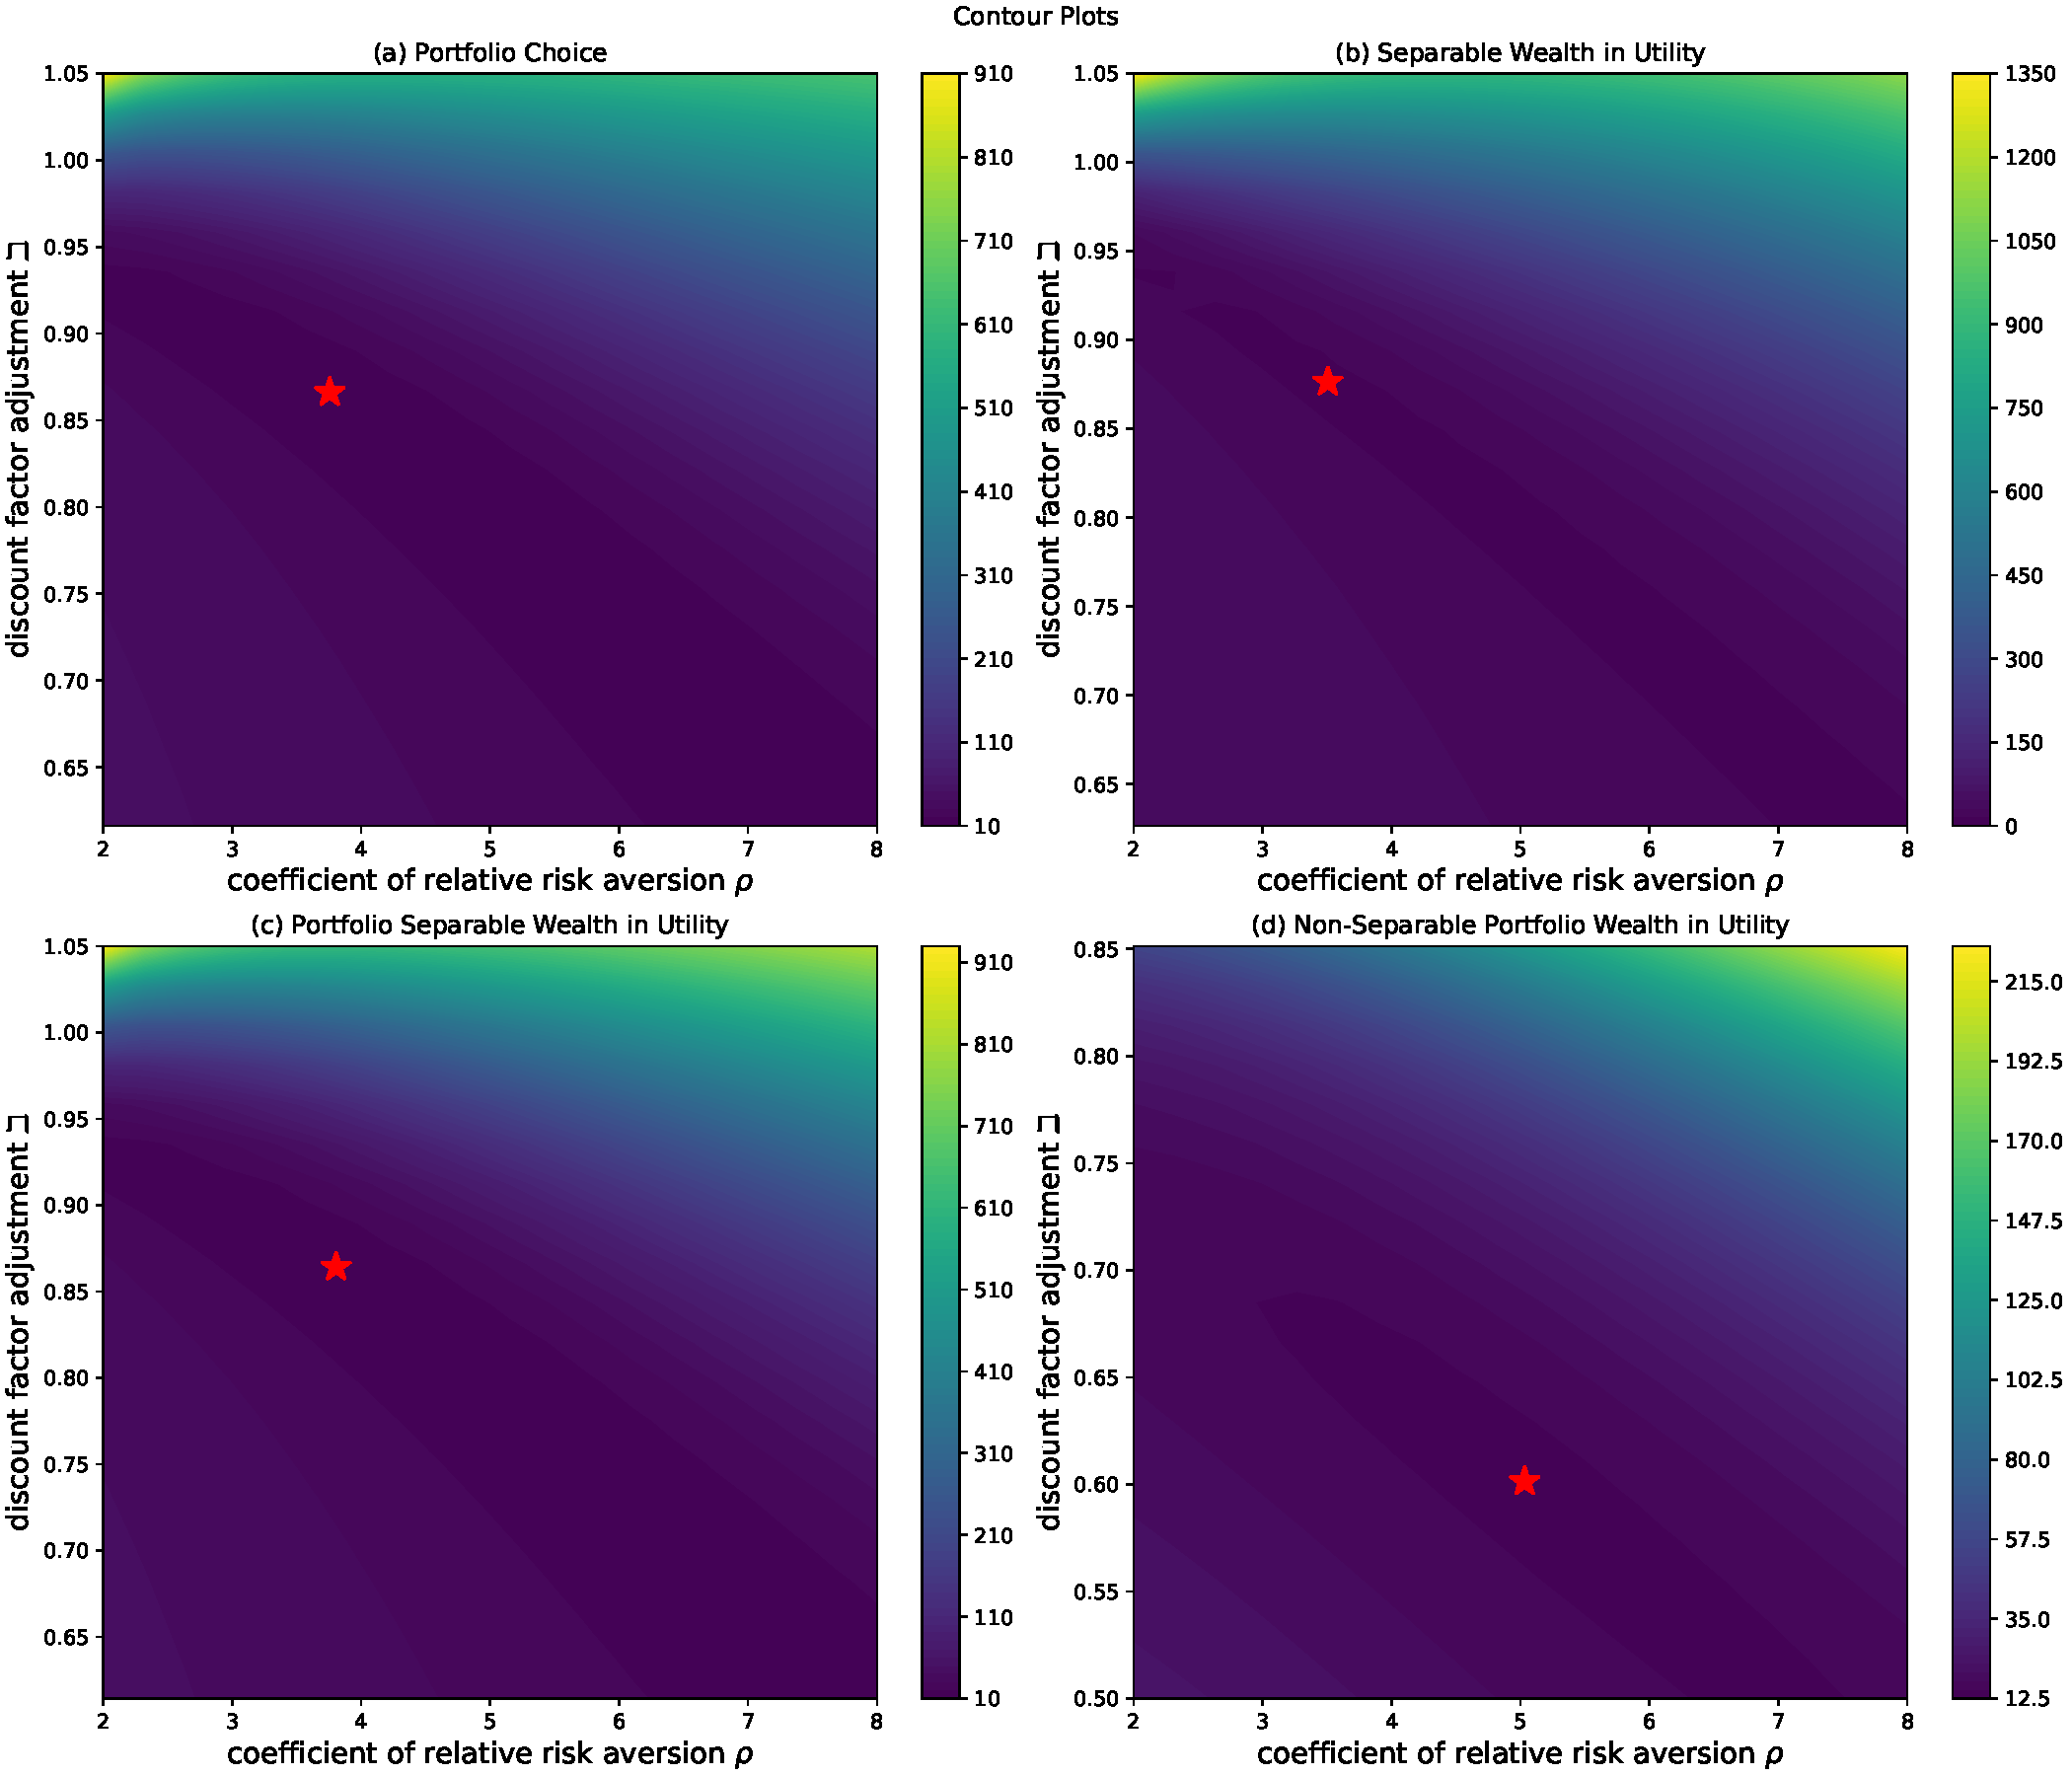
\includegraphics[width=0.7\linewidth]{files/AllSMMcontour-61083533183861c53042688308f7803e.pdf}
\caption{Contour plot of the objective function for the structural estimation of the Life Cycle Incomplete Markets model. The red dot represents the estimated parameters.}
\label{fig:AllSMMcontour}
\end{figure}

\subsection{Sensitivity Analysis}\label{Sensitivity Analysis}

\textbf{Results for LCIM model} For our sensitivity analysis, we use the methods introduced by \cite{Andrews_2017}. Figure~\ref{fig:IndShockSensitivity} shows the sensitivity of the pure discount factor $\beth$ and the coefficient of risk aversion $\CRRA$. As in \cite{Andrews_2017}, the plots are inverses of each other, reflecting the trade-off between the two parameters in fitting lifetime consumption and wealth dynamics. Because the pure discount factor is a multiplicative adjustment on already calibrated life cycle discount factors, the sensitivity analysis has a different interpretation from the one in \cite{Gourinchas_2002}. In our analysis, the adjusted discount factor $\beth$ matters relatively more than $\CRRA$ up to age 40, indicating a potential overshot of the mortality risk and household-adjusted discount factors. For ages 40-50, the sensitivity of $\beth$ and $\CRRA$ is relatively low, indicating that the model is not very sensitive to the values of these parameters in this age range. Finally, from ages 50 and above, the coefficient of relative risk aversion $\CRRA$ matters relatively more than $\beth$. The differences between the sensitivity of this model and that in \cite{Gourinchas_2002} are likely due to the fact that our model uses time-varying discount factors and applies the adjusted discount factor $\beth$ multiplicatively. Thus, it might be that the life cycle discount factors are imprecisely calibrated, which would explain the reversal of the sensitivity of $\beth$ and $\CRRA$ over the life cycle. MOre research is needed to understand this result.

\begin{figure}[!htbp]
\centering
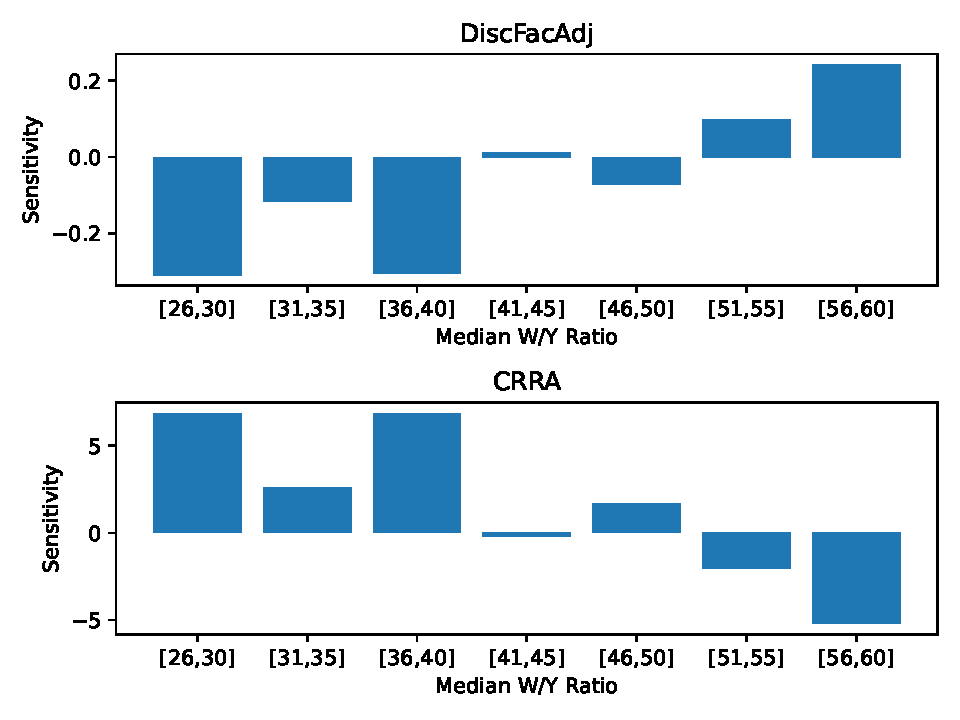
\includegraphics[width=0.7\linewidth]{files/IndShockSensitivity-9046783d8c17a2fc3e39f5fb5ebcf6c7.pdf}
\caption{Sensitivity analysis of the structural estimation of the Life Cycle Incomplete Markets model. The red dot represents the estimated parameters.}
\label{fig:IndShockSensitivity}
\end{figure}

\textbf{Results for WUFIM models} For completeness, Figure~\ref{fig:AllSensitivity} shows the sensitivity analysis for the alternative specifications of the LCIM model. The sensitivity of the Non-Separable WUFIM model appears to diminish in the beginning of the lifecycle, from ages 26-40, and then increases significantly from ages 41-60. This is likely due to the fact that the non-separable WUFIM model has a much higher estimate of the coefficient of relative risk aversion $\CRRA$ than the other models.

\begin{figure}[!htbp]
\centering
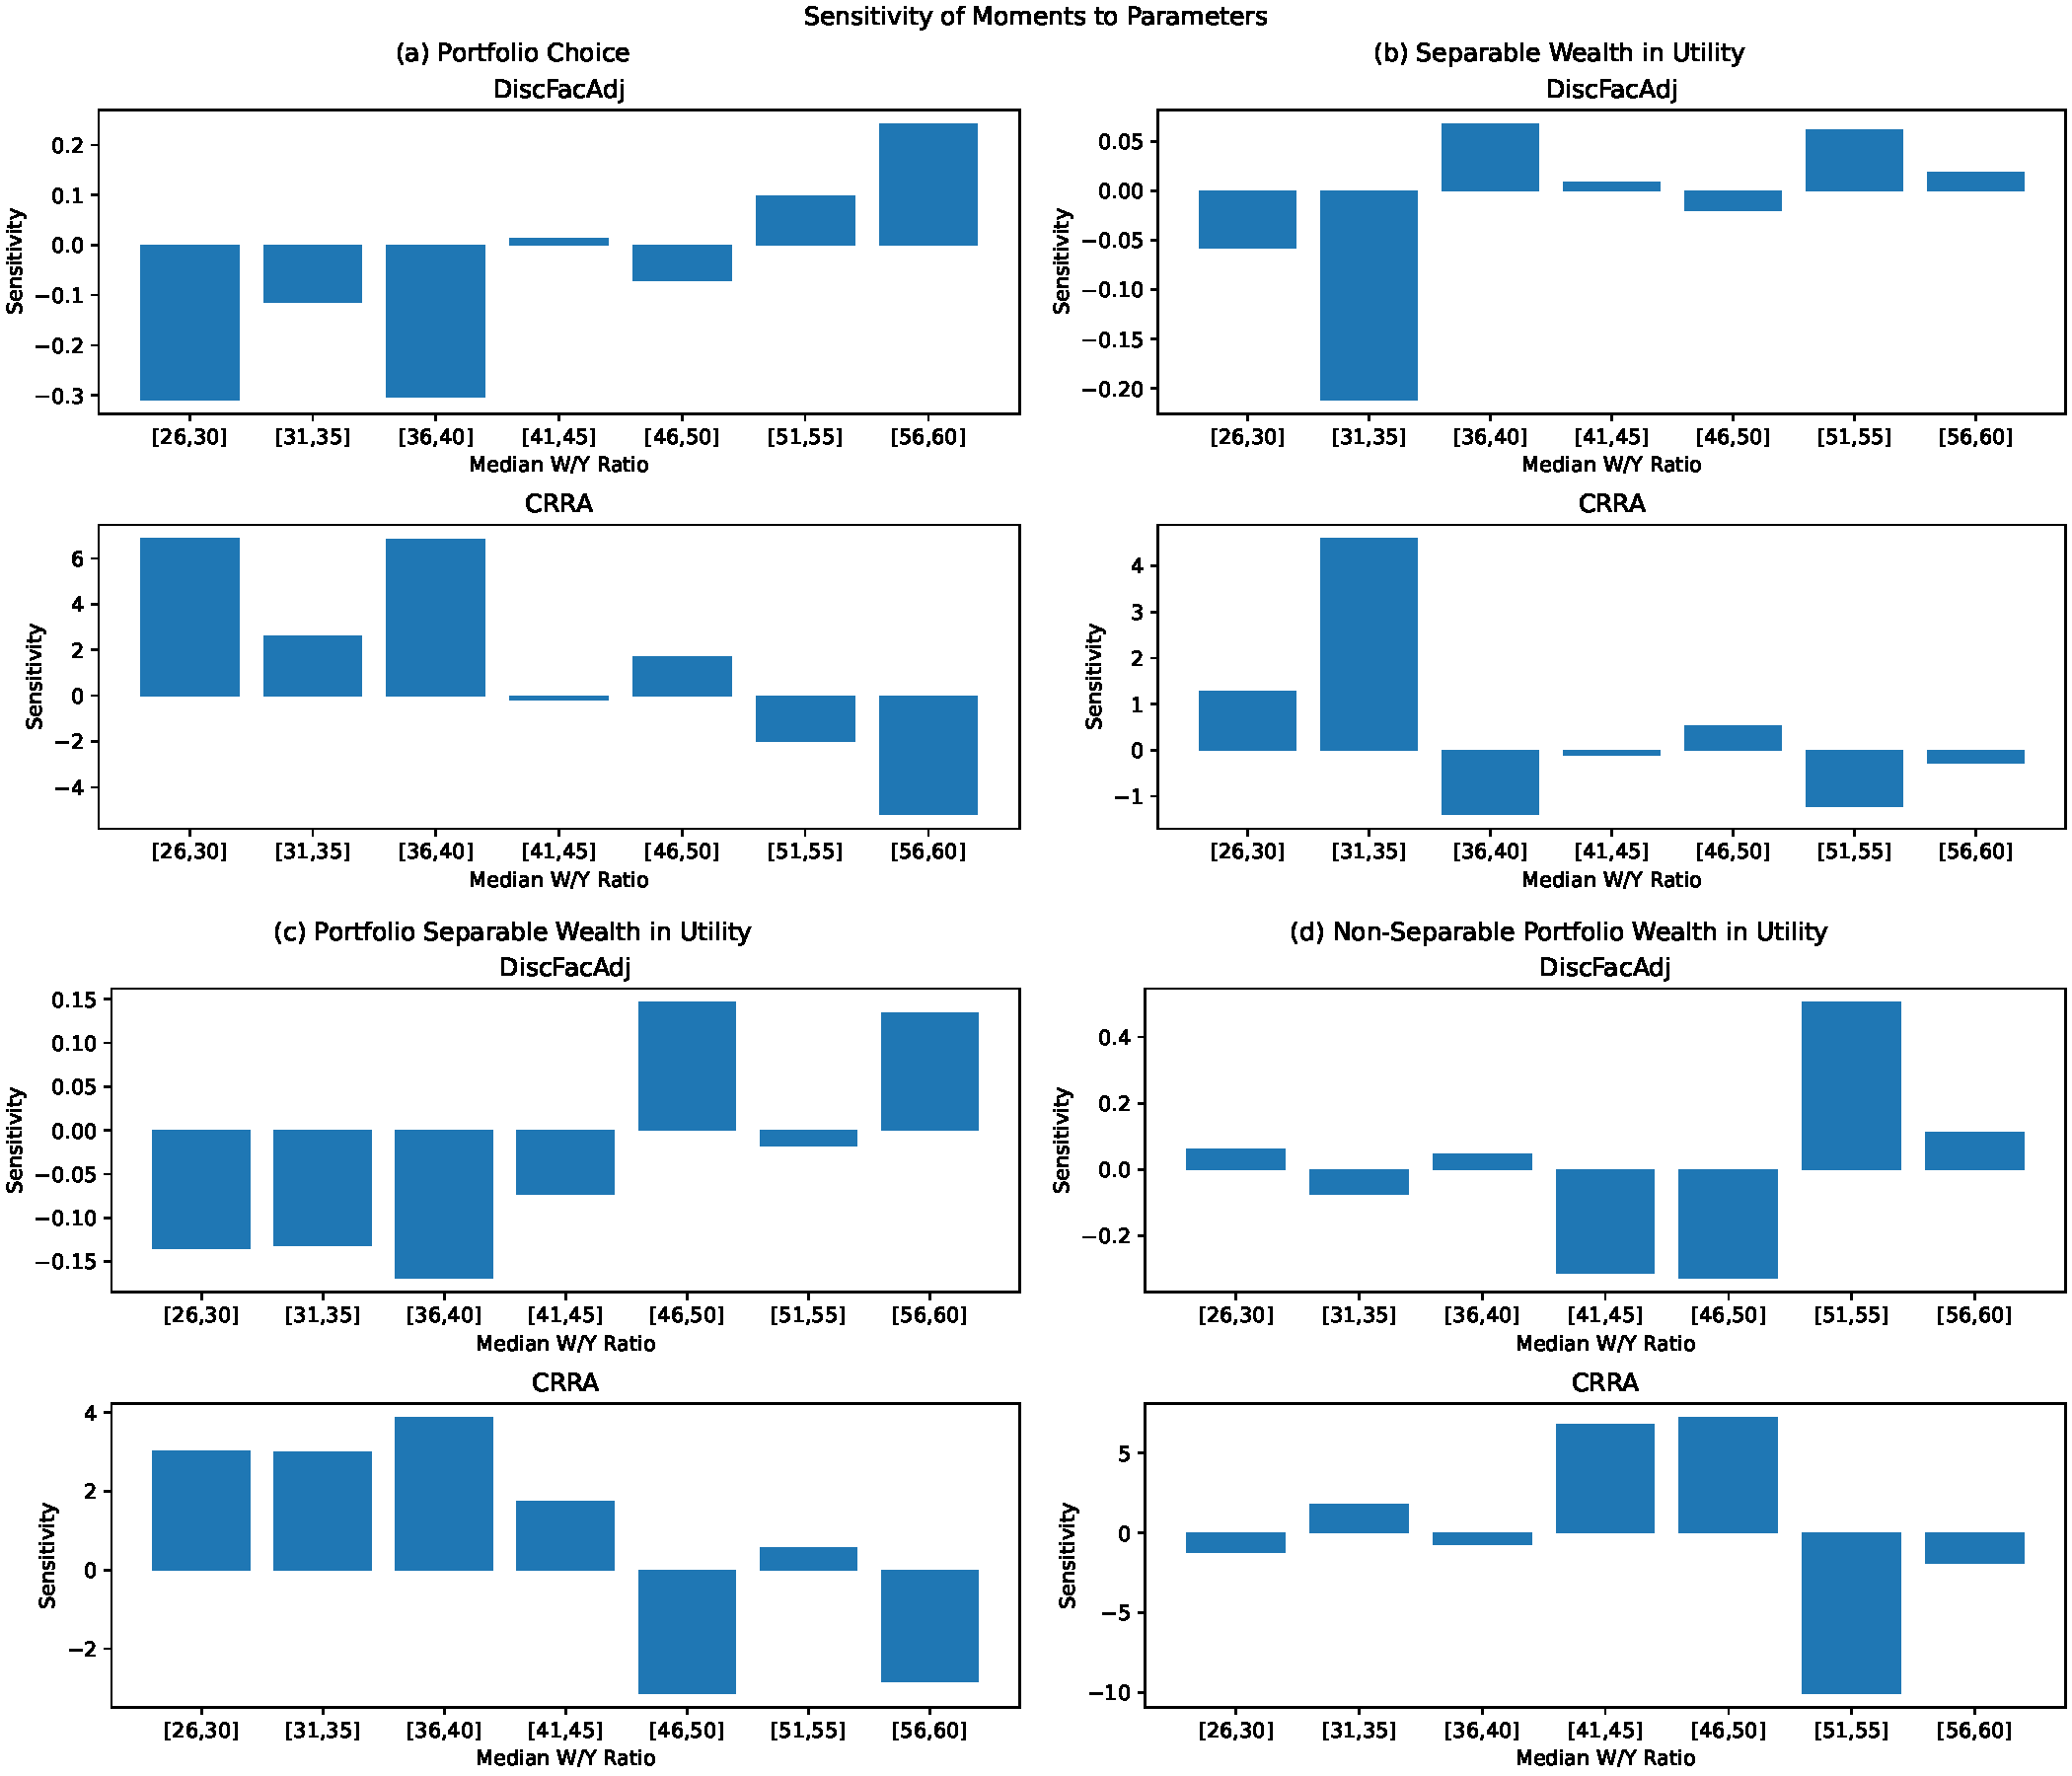
\includegraphics[width=0.7\linewidth]{files/AllSensitivity-0f14236654de527c752f26a13f644a4c.pdf}
\caption{Sensitivity analysis of the structural estimation of the Life Cycle Incomplete Markets model. The red dot represents the estimated parameters.}
\label{fig:AllSensitivity}
\end{figure}

\section{Conclusion}\label{Conclusion}

In this paper, I estimate a Life Cycle Incomplete Markets model with separable and non-separable wealth in the utility function (WUFIM) using the method of simulated moments (SMM) and data from the Survey of Consumer Finances (SCF). I then compare the estimated parameters to those of the standard Life Cycle Incomplete Markets model (LCIM), which is known to be unable to match the distribution of wealth. I find that the estimated parameters for the separable WUFIM model are not very different from those in the LCIM model, which perhaps points at the inability of warm glow and accidental bequest motives to resolve many of the issues of the SIM and LCIM models. The non-separable WUFIM model produces a much lower estimate of the pure discount factor $\beth$ and a significantly higher estimate of the coefficient of risk aversion $\CRRA$. Finally, I conduct sensitivity analysis of the estimated models using the Jacobian of the objective function and find that the sensitivity of the models has the reverse pattern from what we expected. This is because our LCIM and WUFIM models already account for time-varying discount factors due to mortality risk and household size. Thus, the sensitivity analysis is likely picking up on the imprecision of the calibration of the life cycle discount factors.

Further work is needed to understand the implications of these results. First, I will use the mean wealth of each age group instead of the median wealth as the WUFIM models are intended to better match the distribution of wealth. Second, I will evaluate the result of the objective function to see if the WUFIM models are able to match the distribution of wealth better than the LCIM and SIM models. Third, I will use a numerical approximation to the Jacobian of the objective function which will allow for both faster estimation and more accurate sensitivity analysis. Finally, I will use the estimated models to conduct policy analysis and evaluate the welfare implications of macroeconomic shocks.



\bibliographystyle{unsrtnat}
\bibliography{main.bib}

\end{document}
